\subsubsection{Part 3:}

This section again uses larger numbers of users, from 1 to 20, and distances the
users from 0 to 150 meters from the access point.

Due to the large number of outputs from this section, tables, such as that of
Table \ref{tab:QCP3TPTable} are used to show the extracted values from the .db
file.
\begin{figure}[H]
	\centering
	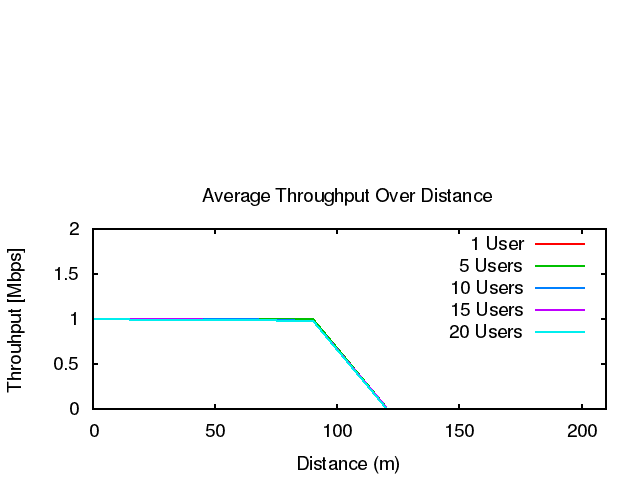
\includegraphics[width=0.8\textwidth]{images/EE500/QC/P3/Images/wifi-throughput}
	\caption{Throughput for systems with 0 to 20 users, over distances from
	0 to 150 meters}
	\label{fig:QCP3throughput}
\end{figure}

The table below shows that for a single user, there is no change in throughput
from 0 to 90 meters, with a large drop at 120 meters. Similarly, for 5 users,
there is only a drop in throughput at a distance of 120 meters.
\par For 10 users,
there is a small decrease in throughput at 90 meters, with a similar large
decrease as before at 120 meters. The 15 user system has a drop in throughput at
60 meters, at 90 meters, and a larger drop again at 120 meters.
\par For 20 users there is an immediate drop at 30 meters, with a slow decrease
in throughput between 30 and 90 meters. Again there is a more dramatic decrease
in throughput at 120 meters.

\begin{table}[H]
	\centering
	\caption{Throughput Values (Kbps) for 1-20 User Systems at Distances of 0-150m}
	\label{tab:QCP3TPTable}
	\begin{tabular}{|c|c|c|c|c|c|}
		\hline
		Distance & 1 User & 5 Users & 10 Users & 15 Users & 20 Users\\
		\hline
		0 & 1000 & 1000 & 1000 & 1000 & 1000\\
		30 & 1000 & 1000 & 1000 & 1000 & 990.8\\
		60 & 1000 & 1000 & 1000 & 986 & 986\\
		90 & 1000 & 1000 & 974.8 & 975.6 & 975.6\\
		120 & 17.6 & 18.4 & 18.4 & 17.6 & 15.2\\
		\hline
	\end{tabular}
\end{table}

\begin{figure}[H]
	\centering
	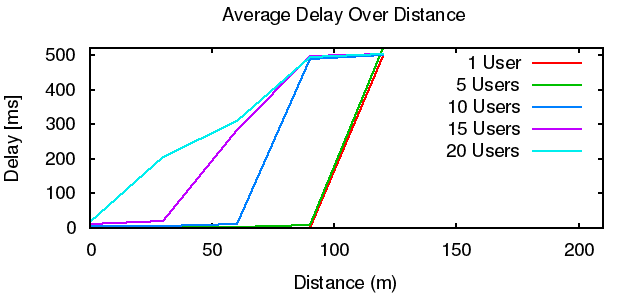
\includegraphics[width=0.8\textwidth]{images/EE500/QC/P3/Images/wifi-delay}
	\caption{Delay for systems with 0 to 20 users, over distances from 0 to
	150 meters}
	\label{fig:QCP3delay}
\end{figure}

For delay, the values have a sharp increase in most cases, for example the
single and five user systems see a large increase at a distance of 120 meters.
The 20 user system however has an initial large increase between 0 and 30
meters, followed by a smaller increase between 30 and 60 meters, followed again
by a large increase between 60 and 90 meters. The final delay value in all cases
is quite similar.

\begin{table}[H]
	\centering
	\caption{Delay Values (ms) for 1-20 User Systems at Distances of 0-150m}
	\label{tab:QCP3TPTable}
	\begin{tabular}{|c|c|c|c|c|c|}
		\hline
		Distance & 1 User & 5 Users & 10 Users & 15 Users & 20 Users\\
		\hline
		0 & 0.194653 & 1.57338 & 5.6031 & 11.2192 & 18.5429\\
		30 & 0.347009 & 2.32888 & 7.16022 & 19.1675 & 203.886\\
		60 & 0.566218 & 3.44795 & 12.5859 & 283.532 & 310.421\\
		90 & 1.27689 & 8.00458 & 488.852 & 496.113 & 494.484\\
		120 & 497.965 & 523.288 & 499.474 & 504.065 & 504.108\\
		\hline
	\end{tabular}
\end{table}

\begin{figure}[H]
	\centering
	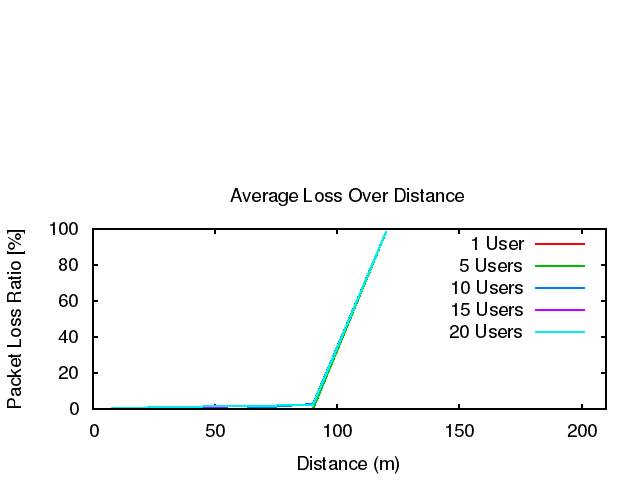
\includegraphics[width=0.8\textwidth]{images/EE500/QC/P3/Images/wifi-loss}
	\caption{Loss for systems with 0 to 20 users, over distances from 0 to
	150 meters}
	\label{fig:QCP3loss}
\end{figure}

Loss can be seen to be similar to the throughput results (due to their
dependence on the number of received packets). All systems have a PLR of
approximately 98\% at a distance of 120 meters. As the number of users
increases, the distance at which loss begins to occur decreases, for example
with 10 users, loss occurs at 90 meters, whereas with 20 users loss occurs at 30
meters.

\begin{table}[H]
	\centering
	\caption{Packet Loss Ratio for 1-20 User Systems at Distances of 0-150m}
	\label{tab:QCP3TPTable}
	\begin{tabular}{|c|c|c|c|c|c|}
		\hline
		Distance & 1 User & 5 Users & 10 Users & 15 Users & 20 Users\\
		\hline
		0 & 0 & 0 & 0 & 0 & 0\\
		30 & 0 & 0 & 0 & 0 & 0.92\\
		60 & 0 & 0 & 0 & 1.4 & 1.4\\
		90 & 0 & 0 & 2.52 & 2.44 & 2.44\\
		120 & 98.24 & 98.16 & 98.16 & 98.24 & 98.48\\
		\hline
	\end{tabular}
\end{table}

From this section, it can be seen that the distance has a greater affect on the
performance characteristics of the system than the number of users, however the
affect of the number of users cannot be discounted
